\documentclass[tikz,border=8pt]{standalone}
% Shared look for every TikZ diagram. Load with \input{../../tools/tikz-style.tex}
\usepackage[T1]{fontenc}
\usepackage{lmodern}
\renewcommand{\sfdefault}{lmr}  % diagrams use the same serif as the text
\usetikzlibrary{arrows.meta, positioning, shapes.geometric, calc, fit, backgrounds}
\definecolor{cblue}{HTML}{4C78A8}
\definecolor{corange}{HTML}{F58518}
\definecolor{cgreen}{HTML}{54A24B}
\definecolor{cred}{HTML}{E45756}
\definecolor{cpurple}{HTML}{B279A2}
\definecolor{cgrey}{HTML}{6B6B6B}
\tikzset{
  every picture/.style={font=\sffamily, line width=1.2pt},
  box/.style={draw=#1, fill=#1!12, rounded corners=4pt, align=center, inner sep=7pt, minimum height=1.1cm},
  box/.default=cgrey,
  arrow/.style={-{Stealth[length=3mm]}, draw=cgrey, line width=1.4pt},
  title/.style={font=\sffamily\bfseries\Large},
  note/.style={font=\sffamily\small, text=cgrey, align=center},
}
\AtBeginDocument{\hyphenpenalty=10000 \exhyphenpenalty=10000}

% One hyperparameter, three names. Numbers from the Note's section 1: n = 1,000 observations.
\begin{document}
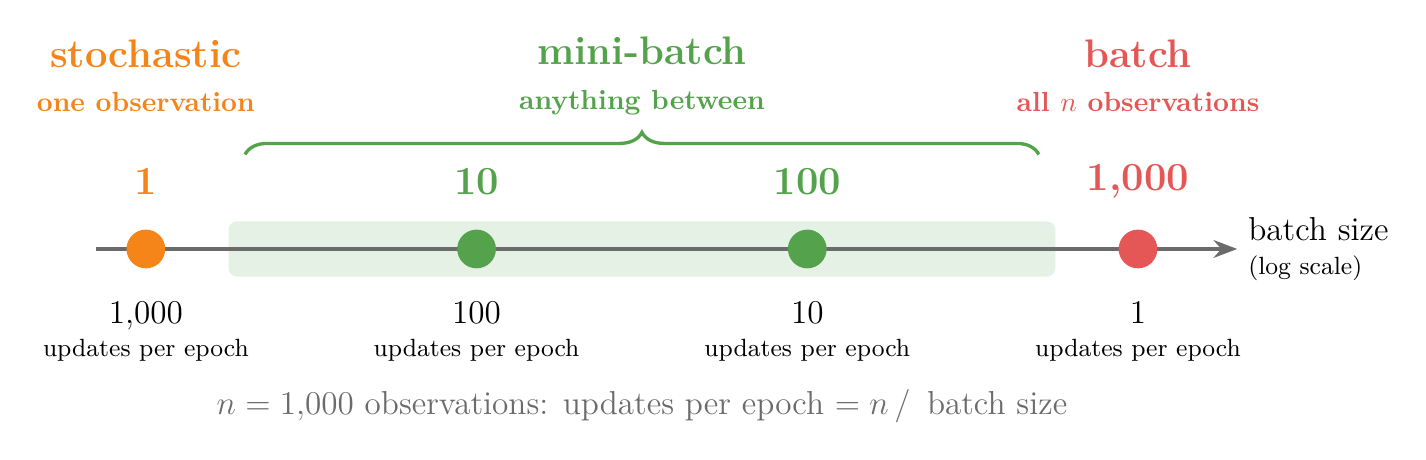
\begin{tikzpicture}[x=4.2cm]
  % log-scale batch-size axis: 1, 10, 100, 1000 at 0..3
  \fill[cgreen!15, rounded corners=3pt] (0.25,-0.35) rectangle (2.75,0.35);
  \draw[arrow] (-0.15,0) -- (3.3,0) node[right, font=\sffamily\large, align=left] {batch size\\[-2pt]{\small (log scale)}};
  \foreach \p/\b/\u/\c in {0/1/1{,}000/corange, 1/10/100/cgreen, 2/100/10/cgreen, 3/1{,}000/1/cred} {
    \fill[\c] (\p,0) circle (7pt);
    \node[font=\sffamily\Large\bfseries, text=\c] at (\p,0.85) {\b};
    \node[font=\sffamily\large, align=center] at (\p,-1.05) {\u\\[-2pt]{\small updates per epoch}};
  }
  \node[font=\sffamily\bfseries\Large, text=corange, align=center] at (0,2.2) {stochastic\\[-2pt]{\normalsize one observation}};
  \node[font=\sffamily\bfseries\Large, text=cgreen, align=center] at (1.5,2.2) {mini-batch\\[-2pt]{\normalsize anything between}};
  \node[font=\sffamily\bfseries\Large, text=cred, align=center] at (3,2.2) {batch\\[-2pt]{\normalsize all $n$ observations}};
  \draw[decorate, decoration={brace, amplitude=8pt}, cgreen] (0.3,1.2) -- (2.7,1.2);
  \node[note, font=\sffamily\large] at (1.5,-2.0) {$n = 1{,}000$ observations: updates per epoch $= n \,/\,$ batch size};
\end{tikzpicture}
\end{document}
